\section{What occupancy counts can tell us about cyclic differences}
\label{sec:geometry}
Why is the search sensitive to a change of coordinates? A useful control is to erase the actual positions at every split and give the optimizer the best local arrangement consistent with the two counts. If the resulting upper bound stays close to the observed recovery, a count-based proof might suffice. If it rises sharply, an accurate obstruction must retain some of the underlying additive geometry. To make the control informative, we first solve the \emph{local} count problem exactly.

\subsection{A sharp one-node bound}
Consider a node of width \(2m\), with \(m\) a power of two. Write its occupied physical even leaves as \(2E\) and its occupied physical odd leaves as \(2O+1\), where \(E,O\subseteq\mathbb Z/m\) have cardinalities \(e,o\). Swapping the names of the physical children only reverses a choice of coordinates. Index an odd increment by \(j\) when it equals \(2j+1\). In the first direction the allowed index set is \(D=O-E\). In the reverse direction it is \(-1-D\). For \(e,o>0\) the exact minimum number of allowed directed odd increments is
\[
 L_m(e,o)=\min\!\left(\{m\}\ \cup\
 \left\{2s\left\lceil
 \frac{\lceil e/s\rceil+\lceil o/s\rceil-1}{2}\right\rceil:
             s\mid m,\ s<m\right\}\right).                  \tag{D}
\]
If either set is empty, the answer is zero. In particular, at width two with both children populated the answer is one. The exceptional full-group term in (D) handles this smallest cycle.

For the lower inequality, let \(H\) be the stabilizer of \(D\) under translation and write \(|H|=s\). If \(H\) is the entire group, \(D\) fills the group. Otherwise \(D\) is a union of cosets of \(H\). In the quotient, Kneser's addition theorem gives at least
\(\lceil e/s\rceil+\lceil o/s\rceil-1\) such cosets. Indeed \(E+H,O+H\) occupy at least the indicated ceiling counts, and \(O-E\) has trivial stabilizer after passing to the quotient. Both \(D\) and its reflected translate are unions of these cosets. Reflection is \(j\mapsto-1-j\) on the quotient of even order. Its fixed-point equation \(2j=-1\) has no solution. Consequently the union of allowed cosets has even size, at least the least even integer above the Kneser lower bound. Multiplication by \(s\) and minimization over possible stabilizers give (D) as a lower bound. \href{https://arxiv.org/abs/1303.3539}{M. DeVos, A short proof of Kneser's addition theorem for abelian groups}.

For attainment, take a minimizing proper divisor \(s\). Set \(a=\lceil e/s\rceil\), \(b=\lceil o/s\rceil\), \(k=a+b-1\), and \(l=\lceil k/2\rceil\). In the quotient, place \(E\) in \(a\) consecutive cosets beginning at zero, and \(O\) in \(b\) consecutive cosets beginning at \(a-1-l\). Their differences lie in the quotient interval from \(-l\) to \(k-l-1\). Both this interval and its reflection fit inside \([-l,l-1]\). In each family fill the cosets until the prescribed number of individual points is reached. Truncating the last coset cannot introduce a new difference. The constructed union has at most \(2ls\) elements. The previously proved lower bound forces equality when \(s\) minimizes (D). If the minimum is \(m\), any sets of the given sizes already attain it by the lower bound. The construction proves a local sharpness statement, simultaneously for all dyadic widths. A family of locally sharp configurations need not glue to a single support.

For example, let \(m=8,e=o=2\). If \(E=O=\{0,4\}\), then \(D=\{0,4\}\) and its reflected translate is \(\{7,3\}\). Four increments are allowed, attaining (D). A one-direction count would have permitted the answer two. It would grant six missing increments when this arrangement has four. Some sets with the same counts have more allowed increments: take \(E=\{0,1\}\) and \(O=\{2,4\}\), with differences \(1,2,3,4\) and reflected indices \(6,5,4,3\). Six of the eight increments are now allowed. The change comes entirely from additive positions. Similarly, one occupied point on each side at width at least four necessarily opens two directed increments. Concentrating both at the cheapest label ranks cannot reverse that fact.

\subsection{From a local theorem to an outer problem}
At every node replace its true missing count by the generous quantity \(d^*=w/2-L_{w/2}(e,o)\). Continue to require an occupied canonical even child in every occupied node. Allow the optimizer to choose the two children's count states, including the orientation, independently of physical coordinates shared with other nodes. For a fixed declared support the numerator has only increased and the denominator is unchanged. Maximizing the relaxed fraction over every possible tree therefore bounds every fixed-label stationary marked construction with rates below a specified cap \(c\).

This apparently modest relaxation has an important order. The variables \(e,o\) count structural leaves, including possible leaves of zero limiting rate in a fixed-support closure. The mass in each child separately enters both \(P\) and \(Q\). A cap does not identify these two numbers. At fixed structural choices and trial level \(z\) the new objective is still linear in the rates, so an optimal closed-box vertex has \(\lfloor64/c\rfloor\) saturated leaves and one residual leaf if \(64/c\) is nonintegral. When the division is exact no residual leaf is needed.

This yields an exact finite recurrence. A state stores the width, number of structural leaves, number of full rates, and presence of the residual rate. To combine two child states, add both optimal child surpluses and
\[
 (2d^*-zw)\bigl(c\,k_{\rm odd}+
                    \rho\,j_{\rm odd}\bigr),\qquad
 \rho=64-c\lfloor64/c\rfloor .
\]
At the leaves include the tail charge \(-za_t\); at the root accept total mass 64. The coefficients of this recurrence are rational at a rational threshold. Updating the threshold to the attained ratio strictly raises it until the maximum surplus is zero. There are only finitely many integer state combinations. This gives the exact optimum of the count relaxation. In particular, independently choosing each best geometry cannot somehow make this an arithmetic lower certificate: each of those best choices was granted to the optimizing player.

\begin{center}\small
\begin{tabular}{@{}rrr@{}}\toprule
Rate cap \(c\)&Both directions, exact upper&Only one direction, percent\\\midrule
\(1\)&\(0\)&0.00\\
\(3/2\)&\(63/788\)&11.28\\
\(2\)&\(20/153\)&49.21\\
\(9/4\)&\(1260/6331\)&49.39\\
\(19/8\)&\(3988/14509\)&49.92\\
\(12/5\)&\(628/2277\)&49.93\\
\(3\)&\(966/2153\)&54.37\\
\(4\)&\(108/205\)&73.77\\
\bottomrule\end{tabular}
\end{center}
\begin{figure}[htbp]\centering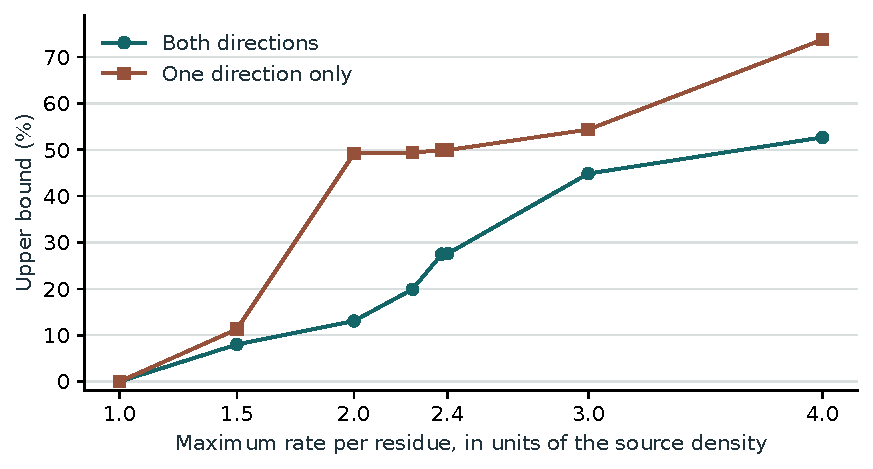
\includegraphics[width=.91\linewidth]{figures/geometry.pdf}
\caption{The exact finite optimum after forgetting joint additive placement. The larger values in the one-direction control quantify a specific accounting error. Neither curve supplies a construction.}\label{fig:geometry}
\end{figure}

\subsection{What survived the erasure}
At \(c=1\) every leaf must be filled at rate one. The vanishing result tests the orientation logic, the total and the possibility of an empty subset. At \(c=2\), the sharp local formula lowers the relaxed ceiling from \(31/63\) to \(20/153\), a change of more than 36 percentage points. At \(12/5\), counting both directions still gives \(628/2277\), roughly \(27.58\%\). The adverse-label enumerations elsewhere in this paper take this far lower. Thus a sharp one-node theorem and every tree occupancy constraint are collectively insufficient for a close estimate at the design cap.

The upper change with \(c\) is also informative. When \(c=2\), at least 32 leaves must carry mass, whereas a cap of \(12/5\) requires only 27. Freeing five leaves creates many opportunities for a difference to disappear. Those opportunities are coupled: omitting a residue to erase one increment changes which preferred minima remain in several other nodes. The separate count recurrence does not pay for incompatible physical placements. This identifies which information a more economical upper proof has to retain.

There is a separate use for a relaxed occupation bound. For a stationary exact-count profile on the conductor-one host, the good-orbit interval sum at a fixed cell bounds each class rate by \(6\mathrm e+o(1)\). To see the rate scale, sum the upper bound \(N_1\) for a window of length \(G'\) over all starting points. Every retained site is then counted \(G'\) times. At fixed depth the cell length greatly exceeds \(G'\), and \(N_1/(G'\delta)\to6\mathrm e\). A cell exceeding this bound by a fixed amount would contribute a positive fraction of the retained set on bad orbits for a positive-weight generator class, contradicting the selector's bad-mass requirement. The prior occupancy study supplies this fixed-depth argument. \href{https://github.com/nousentllc/riemann-hypothesis/pull/10}{Odd-position occupancy study}.

The extra positive-preferred-child condition in this recurrence still matters for the interpretation of that broad comparison. On an occupied long cell with no preferred retained sites, a tile requiring an even mark cannot succeed; a positive-density stationary cell would then contradict the bad-mass condition by the same fixed-depth argument. For stationary exact-count profile families with those occupied preferred children and with all allowed edges realized in the sense of Section~\ref{sec:arithmetic-transport}, \(c=16.31>6\mathrm e\) gives \(34251/39944\), about \(85.75\%\). This deliberately weak number belongs to a wider class. It explains why an upper near ten percent for strict marked profiles cannot simply be promoted to all conceivable source witnesses. A nonstationary hierarchy can evade the fixed-resolution edge-realization description.

The replay exhausts every ordered pair of subsets at group orders \(1,2,4,8\), including all \(65{,}536\) pairs at order eight. It also builds an attaining pair for every one of the \(1{,}497\) occupancy pairs across orders through 32. The first experiment checks the independent lower direction on small instances. The second checks sign conventions in the construction at the actual resolution and exercises every integer input of (D) used in the final calculation.
